\documentclass[mphy386-notes.tex]{subfiles}
\begin{document}
\section{X-ray Image Quality}
In this section we will introduce the basics of x-ray imaging and develop three
tools that we can use to quantify image quality---contrast, resolution, and
noise. We will focus on x-ray imaging in these notes, but these tools are
useful for analyzing all imaging modalities.

\subsection{X-ray Imaging Basics}
We can create an x-ray imaging system by assembling an x-ray \textbf{source}, an
\textbf{object}, and a \textbf{detector}. Figure \ref{fig:simple} shows a simple
example of an x-ray imaging system---we place an x-ray fluence $\bs{\phi}_0$
incident on an object with two attenuation coefficients $\mu_1$ and $\mu_2$. Note that we use bold symbols to indicate random variables.
\begin{figure}[h]
\begin{center}
  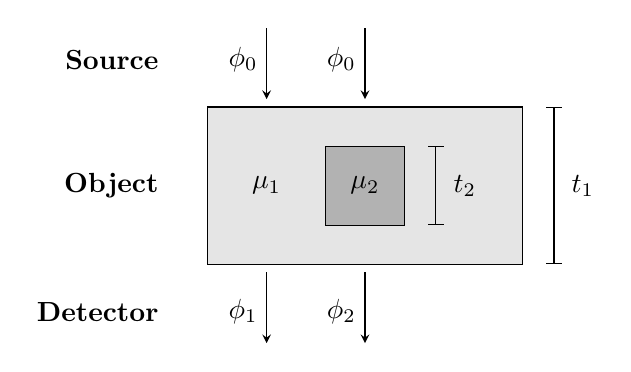
\begin{tikzpicture}[>=stealth]
    \filldraw[fill=black!10!white, draw=black] (-2,-1) rectangle (2,1);
    \filldraw[fill=black!30!white, draw=black] (-0.5,-0.5) rectangle (0.5,0.5);
    \draw [|-|] (2.4,-1) -- (2.4,1);
    \draw [|-|] (0.9,-0.5) -- (0.9,0.5);
    \node[right] at (1.0,0) {$t_2$};
    \node[right] at (2.5,0) {$t_1$};
    \node at (0,0) {$\mu_2$};
    \node at (-1.25,0) {$\mu_1$};
    \draw [->] (-1.25,2) -- (-1.25,1.1);
    \draw [->] (0,2) -- (0,1.1);
    \node at (-1.55,1.6) {$\bs{\phi}_0$};
    \node at (-.3,1.6) {$\bs{\phi}_0$};    
    \draw [->] (-1.25,-1.1) -- (-1.25,-2);
    \draw [->] (0,-1.1) -- (0,-2);
    \node at (-1.55,-1.6) {$\bs{\phi}_1$};
    \node at (-.3,-1.6) {$\bs{\phi}_{2}$};
    \node[left] at (-2.5, 1.6) {\textbf{Source}};
    \node[left] at (-2.5, 0) {\textbf{Object}};
    \node[left] at (-2.5, -1.6) {\textbf{Detector}};    
\end{tikzpicture}
\end{center}
\captionsetup{width=1.0\linewidth}
\caption{Simplified x-ray imaging schematic. A collimated beam of x-rays with
  fluence $\bs{\phi}_o$ is incident on an object with two attenuation
  coefficients. A detector measures the output fluences $\bs{\phi}_{1,2}$.}
\label{fig:simple}
\end{figure}
X-rays are attenuated as they pass through the object so the exit fluences are
related to the input fluence by
\begin{align}
  \bs{\phi}_1 &= \bs{\phi}_0e^{-\mu_1 t_1}\\
  \bs{\phi}_2 &= \bs{\phi}_0e^{-\mu_1(t_1 - t_2) - \mu_2t_2}. 
\end{align}
When we place a detector in the path of the exit beam we create an image of the
object. 

We will examine more realistic sources and detectors in later sections, but the
simple example in Figure \ref{fig:simple} is sufficient for us to model image
quality in x-ray imaging systems. 

\subsection{Rose Model}
Suppose that we'd like to detect the presence or absence of the small object
with attenuation $\mu_2$ in Figure \ref{fig:simple} with our imaging system. How
well can we perform this task? What conditions do we need to meet to confidently
say that the object is present or absent? How should we design our imaging
system to meet these conditions? The Rose model supplies answers to these
questions and gives us a solid framework for understanding image quality.

First, we define the \textbf{signal} $S$ as the mean number of photons
blocked by the object
\begin{align}
  S \equiv A(\text{E}\{\bs{\phi}_1\} - \text{E}\{\bs{\phi}_2\}) = A\Delta\phi
\end{align}
where $A$ is the cross sectional area of the object, $\text{E}\{\cdot\}$ denotes
the expectation value, $\phi$ is the x-ray fluence in units of photons per unit
area, and $\Delta\phi \equiv \text{E}\{\bs{\phi}_1\} -
\text{E}\{\bs{\phi}_2\}$. This may seem like a peculiar way to define the
signal---shouldn't the signal be the measured intensity difference between areas
with and without the object? The reason for our definition is that it captures
the role of object size in detectability. Intuitively, larger objects are easier
to detect, so our definition of signal should reflect this.

Next, we consider the \textbf{noise} $N$ that corrupts our signal. Note that in
signal-to-noise ratio discussions the word ``noise'' usually refers to the
standard deviation of a random variable. We will use this meaning. In general
the word ``noise'' refers to any random or unwanted signals.

We define the noise as the standard deviation of the number of photons detected
in an area the size of the object when the object is absent. 
\begin{align}
  N &\equiv \sqrt{\text{Var}\{A\bs{\phi}_1\}}.\\
  \intertext{$A\bs{\phi}_1$ is a Poisson-distributed random variable, so its variance is identical to its mean}
  N &= \sqrt{\text{E}\{A\bs{\phi}_1\}}\\
  N &= \sqrt{A\text{E}\{\bs{\phi}_1\}}.
\end{align}

Finally, the signal-to-noise ratio is given by
 \begin{align}
   \text{SNR} &\equiv \frac{S}{N} = \frac{A\Delta\phi}{\sqrt{AE\{\bs{\phi}_1\}}}
 \end{align}   
% %  \text{SNR} &= C\sqrt{A\bar{\phi}} 

where $C$ is the radiation contrast:
\begin{align}
  C = \frac{\Delta\phi}{\bar{\phi}}
\end{align}
This is the SNR for an ideal detector where we've assumed that
\begin{itemize}
\item complete absorption of incident quanta
\item no added noise
\item no loss of spatial resolution (i.e., no blurring)
\end{itemize}

\fig{img/contrast.png}{.25}{Test}{constrast}

\pagebreak
\end{document}